% L2OSobolev: masked Sobolev supervision as a regularizer on any method.
%
% Dataset: each sampled p_i is solved (S1) for the value label g(p_i); a
% sensitivity oracle (DiffOpt, implicit differentiation of the KKT conditions
% (S3), or finite differences) gives the derivative label Dg(p_i).
% Training: the proxy g-hat_theta enters the inner method's loss (any method;
% value matching for supervised methods); its input Jacobian, masked by M,
% is matched to the masked label (S5); the total loss is (S4).
% The layout follows Fig. 1 of the masked Sobolev paper (NeurIPS 2026);
% notation follows docs/src/sobolev/theory.md.
%
% Build: make -C docs/src/assets/diagrams/src
%   pdflatex -jobname=l2osobolev--regularizer sobolev.tex          -> wide layout
%   pdflatex -jobname=l2osobolev--regularizer-compact sobolev.tex  -> narrow layout
\documentclass[tikz,border=4pt]{standalone}
% Shared style of the LearningToOptimize diagrams: the palette, lane frames, cards,
% chips and glyphs of the paper-style TikZ figures (the same visual system as the
% PortfolioOpt.jl and DecisionRules.jl figures). Each figure \input's this file.
\usepackage{amsmath,amssymb,bm}
\usepackage[T1]{fontenc}
\usepackage[scaled=0.92]{helvet}
\renewcommand{\familydefault}{\sfdefault}
\usetikzlibrary{arrows.meta,shapes.geometric,shapes.symbols,calc,positioning,decorations.pathreplacing}

\definecolor{dTeal}{HTML}{1A9AA0}
\definecolor{dTealLine}{HTML}{3FB3B8}
\definecolor{dNavy}{HTML}{3F4C8C}
\definecolor{dInk}{HTML}{1E2235}
\definecolor{dRed}{HTML}{E4573D}
\definecolor{dCoral}{HTML}{E2765A}
\definecolor{dOrange}{HTML}{F4A93B}
\definecolor{dPeach}{HTML}{FBD9AC}
\definecolor{dPanel}{HTML}{EEF0F2}
\definecolor{dGray}{HTML}{8A90A0}
\definecolor{dNode}{HTML}{14A3A8}
\definecolor{dShadow}{HTML}{D5DAE3}

% \ifcompact is true when the job name ends in "-compact" (narrow layout).
\newif\ifcompact
\ifnum\pdfmatch{-compact$}{\jobname}=1 \compacttrue\fi

\tikzset{
  >={Stealth[length=5pt,width=4pt]},
  every node/.style={text=dInk},
  title/.style={anchor=west,font=\small,inner sep=0pt},
  head/.style={font=\small\bfseries,text=dNavy},
  note/.style={font=\itshape\footnotesize,text=dNavy},
  dnote/.style={font=\itshape\footnotesize,text=dCoral},
  code/.style={font=\ttfamily\footnotesize,text=dNavy},
  store/.style={cylinder,shape border rotate=90,aspect=0.28,fill=dPeach,draw=dOrange,
                line width=0.7pt,minimum width=0.95cm,minimum height=1.2cm,font=\normalsize},
  dia/.style={diamond,fill=dOrange,draw=none,minimum size=0.9cm,inner sep=0pt,aspect=1,
              font=\normalsize},
  lnode/.style={circle,fill=dRed,draw=none,minimum size=0.66cm,inner sep=1pt,
                text=white,font=\normalsize},
  card/.style={rectangle,rounded corners=4pt,fill=white,draw=dShadow,line width=0.6pt},
  sheet/.style={rectangle,rounded corners=3pt,fill=dPanel,draw=dShadow,line width=0.6pt},
  chip/.style={rectangle,rounded corners=3pt,fill=dPanel,draw=none,font=\small,
               inner xsep=4pt,inner ysep=3pt},
  ochip/.style={chip,fill=white,draw=dGray,dashed,line width=0.6pt},
  pchip/.style={chip,fill=white,draw=dGray!70,dashed,line width=0.5pt,text=dGray},
  fwd/.style={->,dTealLine,line width=0.8pt},
  tgt/.style={->,dOrange,line width=0.9pt},
  dual/.style={->,dCoral,dashed,line width=0.9pt},
  dep/.style={->,dTealLine,line width=0.8pt},
  pdep/.style={->,dGray,dashed,line width=0.7pt},
  nn/.style={circle,minimum size=0.26cm,inner sep=0pt,draw=dInk!70,line width=0.35pt},
}

% Lane frame in the paper style: two shadow copies behind a teal rounded frame.
\newcommand{\lane}[4]{% #1 x0, #2 y0, #3 x1, #4 y1
  \foreach \o/\c in {0.16/dShadow!60,0.08/dShadow}
    \draw[\c,fill=white,rounded corners=5pt,line width=0.6pt]
      (#1+\o,#2-\o) rectangle (#3+\o,#4-\o);
  \draw[dTealLine,fill=white,rounded corners=5pt,line width=0.9pt] (#1,#2) rectangle (#3,#4);}

% Plain card frame (no shadow copies), for problems and losses.
\newcommand{\cardbox}[4]{\draw[dShadow,fill=white,rounded corners=4pt,line width=0.6pt] (#1,#2) rectangle (#3,#4);}

% Network glyph on one sheet. #1 = centre, #2 = name prefix, #3 = number of stacked
% sheets behind (0, 1 or 2).
\newcommand{\net}[3]{%
  \begin{scope}[shift={(#1)}]
    \ifnum#3>1 \node[sheet,minimum width=1.9cm,minimum height=1.8cm] at (0.30,0.22) {};\fi
    \ifnum#3>0 \node[sheet,minimum width=1.9cm,minimum height=1.8cm] at (0.15,0.11) {};\fi
    \node[sheet,minimum width=1.9cm,minimum height=1.8cm,fill=white] (#2sheet) at (0,0) {};
    \foreach \y [count=\i] in {0.36,0,-0.36} \node[nn,fill=dGray!45] (#2in\i) at (-0.64,\y) {};
    \foreach \y [count=\i] in {0.58,0.29,0,-0.29,-0.58} \node[nn,fill=dNode] (#2ha\i) at (-0.21,\y) {};
    \foreach \y [count=\i] in {0.44,0.15,-0.15,-0.44} \node[nn,fill=dNode] (#2hb\i) at (0.21,\y) {};
    \node[nn,fill=dOrange] (#2out) at (0.64,0) {};
    \foreach \a in {1,...,3} \foreach \b in {1,...,5} \draw[dGray!60,line width=0.2pt] (#2in\a) -- (#2ha\b);
    \foreach \a in {1,...,5} \foreach \b in {1,...,4} \draw[dGray!60,line width=0.2pt] (#2ha\a) -- (#2hb\b);
    \foreach \a in {1,...,4} \draw[dGray!60,line width=0.2pt] (#2hb\a) -- (#2out);
  \end{scope}}

% Jacobian mask glyph: an n x d grid with a few entries selected. #1 = centre.
\newcommand{\maskgrid}[1]{%
  \begin{scope}[shift={(#1)}]
    \foreach \i in {0,...,4} \foreach \j in {0,...,3}
      \draw[dShadow,fill=white,line width=0.4pt] (\j*0.2-0.4,-\i*0.2+0.5) rectangle ++(0.2,-0.2);
    \foreach \i/\j in {0/1,1/3,2/0,3/2,4/1}
      \draw[dOrange,fill=dOrange,line width=0.4pt] (\j*0.2-0.4,-\i*0.2+0.5) rectangle ++(0.2,-0.2);
  \end{scope}}

% Code names inside italic notes stay upright.
\newcommand{\cmd}[1]{{\upshape\ttfamily #1}}

% Software-architecture helpers: package cards, type chips and chip rows.
\tikzset{
  pkg/.style={rectangle,rounded corners=4pt,fill=white,draw=dShadow,line width=0.6pt,
              align=center,inner xsep=5pt,inner ysep=4pt,font=\footnotesize},
  pkgcore/.style={pkg,draw=dTealLine,line width=0.9pt},
  pkgplan/.style={pkg,draw=dGray,dashed,text=dGray},
  tchip/.style={chip,font=\ttfamily\footnotesize,inner xsep=3pt,inner ysep=2.5pt},
  tplan/.style={tchip,fill=white,draw=dGray,dashed,line width=0.5pt,text=dGray},
  absname/.style={anchor=west,font=\ttfamily\footnotesize,text=dNavy,inner sep=1pt},
}
% \chiprow{x}{y}{style}{A,B,C}: chips left to right from (x,y), anchored west.
\newcommand{\chiprow}[4]{%
  \coordinate (cr@next) at (#1,#2);
  \foreach \t in {#4} {%
    \node[#3,anchor=west] (cr@last) at (cr@next) {\t};
    \coordinate (cr@next) at ($(cr@last.east)+(0.12,0)$);}}


\newcommand{\solve}{%
  $\begin{aligned}
    g(p_i)=x^\star(p_i)\in\;&\arg\min_{x}\;\; f(x;p_i)\\[1pt]
    &\;\text{s.t.}\;\; c(x;p_i)=0,\\
    &\;\phantom{\text{s.t.}}\;\; h(x;p_i)\le 0
  \end{aligned}$}
\newcommand{\masked}{%
  $\begin{aligned}
    \ell_d\big(&\mathcal{M}\odot D\hat g_\theta(p_i),\\
    &\mathcal{M}\odot Dg(p_i)\big)\;\;\text{(S5)}
  \end{aligned}$}
\newcommand{\total}{$\mathcal{L}(\theta)=\text{inner loss}\;+\;\lambda\,\tfrac1N\textstyle\sum_i\ell_d$\;\;(S4)}

\begin{document}
\ifcompact
% ============================ narrow (phone) layout ============================
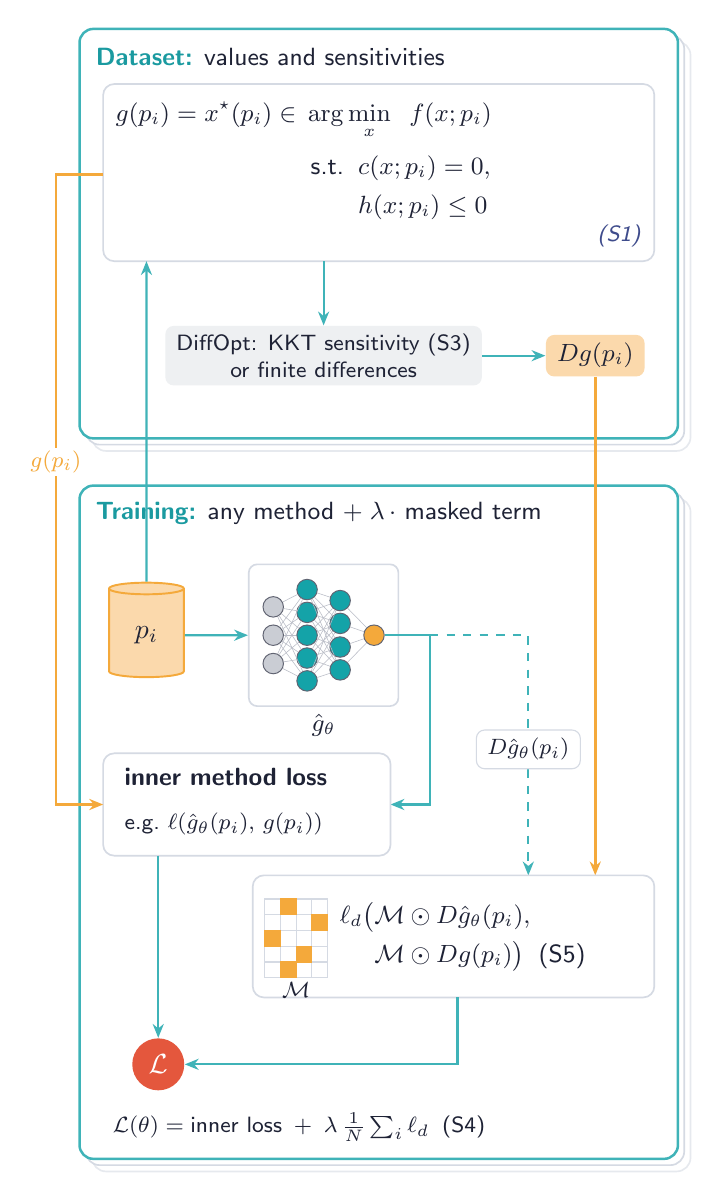
\begin{tikzpicture}
  % ---- dataset ----
  \lane{0}{8.4}{7.6}{13.6}
  \node[title] at (0.2,13.25) {\textcolor{dTeal}{\bfseries Dataset:} values and sensitivities};
  \cardbox{0.3}{10.65}{7.3}{12.9}
  \node[anchor=north west,font=\small,inner sep=0pt] at (0.45,12.7) {\solve};
  \node[note,anchor=south east] at (7.25,10.7) {(S1)};
  \node[chip,align=center,font=\footnotesize] (or) at (3.1,9.45) {DiffOpt: KKT sensitivity (S3)\\or finite differences};
  \draw[fwd] (3.1,10.65) -- (or.north);
  \node[chip,fill=dPeach] (dg) at (6.55,9.45) {$Dg(p_i)$};
  \draw[fwd] (or.east) -- (dg.west);
  % ---- training ----
  \lane{0}{-0.75}{7.6}{7.8}
  \node[title] at (0.2,7.45) {\textcolor{dTeal}{\bfseries Training:} any method $+\;\lambda\,\cdot$ masked term};
  \node[store] (p) at (0.85,5.9) {$p_i$};
  \draw[fwd] (p.north) -- (0.85,10.65);
  \net{3.1,5.9}{px}{0}
  \node[font=\small] at (3.1,4.75) {$\hat g_\theta$};
  \draw[fwd] (p.east) -- (pxsheet.west);
  \coordinate (fk) at (4.45,5.9);
  \draw[fwd] (pxout.east) -- (fk) -- (4.45,3.75) -- (3.95,3.75);
  % inner loss
  \cardbox{0.3}{3.1}{3.95}{4.4}
  \node[font=\small\bfseries,anchor=west] at (0.45,4.1) {inner method loss};
  \node[font=\footnotesize,anchor=west] at (0.45,3.5) {e.g.\ $\ell(\hat g_\theta(p_i),\,g(p_i))$};
  % value label from the dataset, around the left
  \draw[tgt] (0.3,11.75) -- (-0.3,11.75) -- (-0.3,3.75) -- (0.3,3.75);
  \node[font=\footnotesize,text=dOrange,fill=white,inner sep=1pt] at (-0.3,8.1) {$g(p_i)$};
  % derivative path
  \draw[fwd,dashed] (fk) -- (5.7,5.9) -- (5.7,2.85);
  \node[chip,fill=white,draw=dShadow,font=\footnotesize] at (5.7,4.45) {$D\hat g_\theta(p_i)$};
  \draw[tgt] (dg.south) -- (6.55,2.85);
  % masked term
  \cardbox{2.2}{1.3}{7.3}{2.85}
  \maskgrid{2.75,2.05}
  \node[font=\footnotesize] at (2.75,1.4) {$\mathcal{M}$};
  \node[anchor=west,font=\small,inner sep=0pt] at (3.3,2.07) {\masked};
  % total
  \node[lnode] (L) at (1.0,0.45) {$\mathcal{L}$};
  \draw[fwd] (1.0,3.1) -- (L.north);
  \draw[fwd] (4.8,1.3) -- (4.8,0.45) -- (L.east);
  \node[font=\footnotesize,anchor=west] at (0.3,-0.35) {\total};
\end{tikzpicture}
\else
% =============================== wide layout ===================================
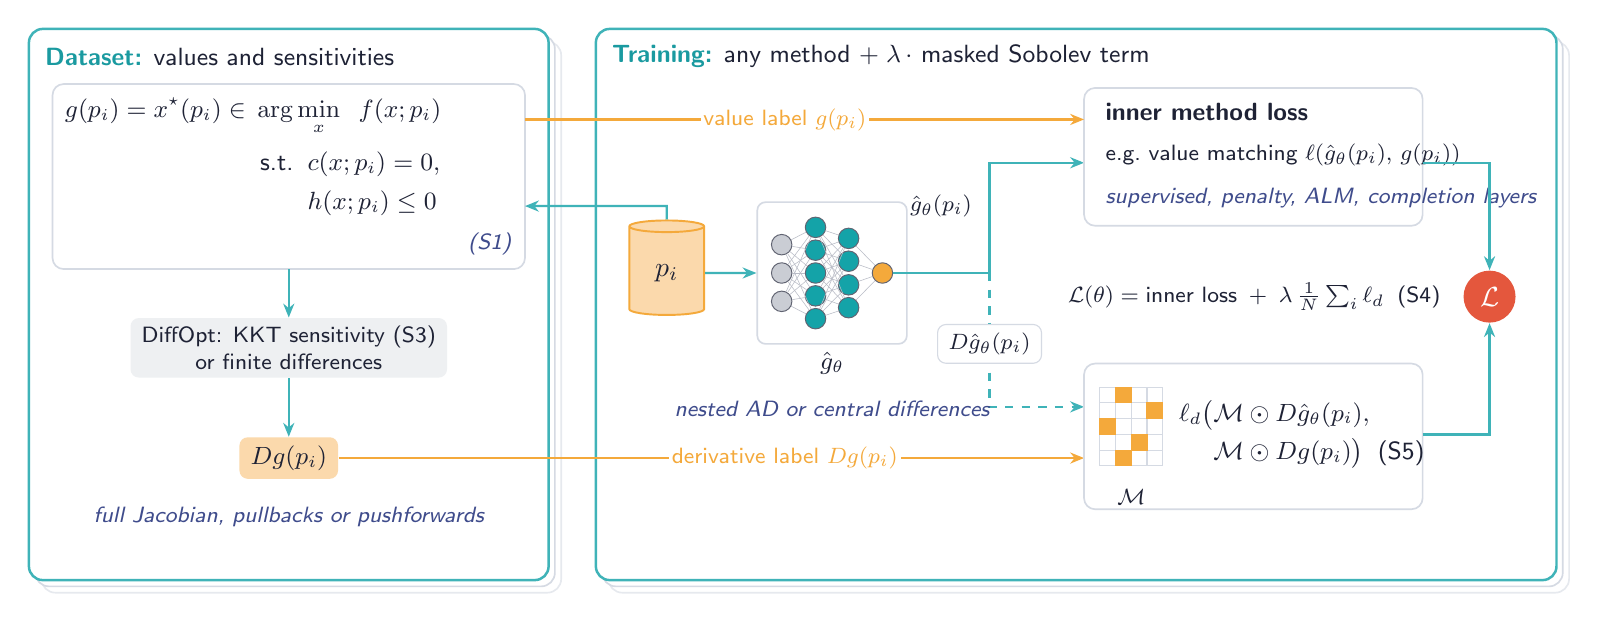
\begin{tikzpicture}
  % ---- dataset ----
  \lane{0}{0}{6.6}{7.0}
  \node[title] at (0.2,6.65) {\textcolor{dTeal}{\bfseries Dataset:} values and sensitivities};
  \cardbox{0.3}{3.95}{6.3}{6.3}
  \node[anchor=north west,font=\small,inner sep=0pt] at (0.45,6.15) {\solve};
  \node[note,anchor=south east] at (6.25,4.0) {(S1)};
  \node[chip,align=center,font=\footnotesize] (or) at (3.3,2.95) {DiffOpt: KKT sensitivity (S3)\\or finite differences};
  \draw[fwd] (3.3,3.95) -- (or.north);
  \node[chip,fill=dPeach] (dg) at (3.3,1.55) {$Dg(p_i)$};
  \draw[fwd] (or.south) -- (dg.north);
  \node[note] at (3.3,0.8) {full Jacobian, pullbacks or pushforwards};

  % ---- training ----
  \lane{7.2}{0}{19.4}{7.0}
  \node[title] at (7.4,6.65) {\textcolor{dTeal}{\bfseries Training:} any method $+\;\lambda\,\cdot$ masked Sobolev term};
  \node[store] (p) at (8.1,3.9) {$p_i$};
  \draw[fwd] (p.north) -- (8.1,4.75) -- (6.3,4.75);
  \net{10.2,3.9}{px}{0}
  \node[font=\small] at (10.2,2.75) {$\hat g_\theta$};
  \draw[fwd] (p.east) -- (pxsheet.west);
  \coordinate (fk) at (12.2,3.9);
  \draw[fwd] (pxout.east) -- (fk) -- (12.2,5.3) -- (13.4,5.3);
  \node[font=\footnotesize,anchor=east] at (12.1,4.75) {$\hat g_\theta(p_i)$};
  % inner loss
  \cardbox{13.4}{4.5}{17.7}{6.25}
  \node[font=\small\bfseries,anchor=west] at (13.55,5.95) {inner method loss};
  \node[font=\footnotesize,anchor=west] at (13.55,5.4) {e.g.\ value matching $\ell(\hat g_\theta(p_i),\,g(p_i))$};
  \node[note,anchor=west] at (13.55,4.85) {supervised, penalty, ALM, completion layers};
  % value label
  \draw[tgt] (6.3,5.85) -- (13.4,5.85);
  \node[font=\footnotesize,text=dOrange,fill=white,inner sep=1pt] at (9.6,5.85) {value label $g(p_i)$};
  % derivative path
  \draw[fwd,dashed] (fk) -- (12.2,2.2) -- (13.4,2.2);
  \node[chip,fill=white,draw=dShadow,font=\footnotesize] at (12.2,3.0) {$D\hat g_\theta(p_i)$};
  \node[note,anchor=north] at (10.2,2.4) {nested AD or central differences};
  \draw[tgt] (dg.east) -- (13.4,1.55);
  \node[font=\footnotesize,text=dOrange,fill=white,inner sep=1pt] at (9.6,1.55) {derivative label $Dg(p_i)$};
  % masked term
  \cardbox{13.4}{0.9}{17.7}{2.75}
  \maskgrid{14.0,1.95}
  \node[font=\footnotesize] at (14.0,1.05) {$\mathcal{M}$};
  \node[anchor=west,font=\small,inner sep=0pt] at (14.6,1.85) {\masked};
  % total
  \node[lnode] (L) at (18.55,3.6) {$\mathcal{L}$};
  \draw[fwd] (17.7,5.3) -| (L.north);
  \draw[fwd] (17.7,1.85) -| (L.south);
  \node[font=\footnotesize,anchor=east] at (18.05,3.6) {\total};
\end{tikzpicture}
\fi
\end{document}
